\section{Mediciones y Experimentos}

Para poder realizar las mediciones utilizamos la instrucción de assembler \textit{rdtsc}. Con ella podemos obtener el valor de Time Stamp Counter (TSC) del procesador -un registro de 64 bits presente en todos los procesadores x86 desde los Pentium-, como este se incrementa en uno con cada ciclo del procesador podemos obtener la duración en cantidad de ticks de una llamada a una función calculando la diferencia de este registro al principio y al final de su ejecución. Ya que esta medida no es constante entre llamadas, por cada caso de test se realizaron 1000 llamadas y se las promedió utilizando el framework provisto por la cátedra. Para lidiar con los posibles outliers se calculó una media 10\% podada. Otros detalles de las mediciones se dan específicamente por cada experimento producido.

\subsection{Performance}

Nos propusimos observar el crecimiento en la cantidad de ciclos por llamada de cada función a medida que crecía el tamaño del archivo de entrada. Para esto utilizamos la imagen de Lena con tamaños de 16x16 píxeles hasta 1024x1024 en incrementos de a 8 píxeles por lado -para el filtro Blit las mediciones arrancaron con imágenes de 128x128 dadas las restricciones del filtro-. El objetivo de estos tests es comparar la performance de la implementación de cada filtro en un lenguaje de alto nivel como C y en uno de nivel más bajo como Assembler. Sabemos que la programación en bajo nivel provee poca -o ninguna- abstracción del set de instrucciones de una arquitectura, debido a esta cercanía del código con el procesador podríamos esperar que la ejecución sea más rápida y que fuese más eficiente en el uso de la memoria. Por el lado del código en C, hicimos las mediciones compilando con los flags O0 y O3 para observar en mayor detalle las variaciones en performance.

En todos los resultados obtenidos observamos que nuestra implementación en ASM requirió menos ciclos de reloj que su contraparte en C en cualquiera de sus variantes. Al mismo tiempo no observamos diferencias notorias entre compilar el código en C usando los flags O0 y O3, al menos no en comparación a la difererencia con el código en assembly. 

Las diferencias registradas en cada implementación son coherentes con el diseño de los algoritmos dadas las posibilidades de cada paradigma de programación: mientras que en los casos de la programación en alto nivel con C toda la programación la realizamos secuencialmente procesando de a un píxel, en bajo nivel con ASM podemos procesar múltiples píxeles con pocas instrucciones SIMD, acortando significativamente la cantidad de ciclos.

\begin{wrapfigure}{r}{0.3\textwidth}
	\centering
	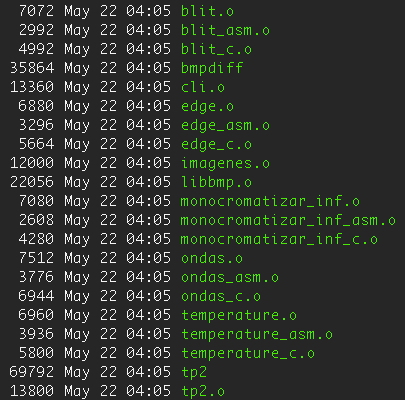
\includegraphics[width=0.3\textwidth]{imagenes/testperformance/sizes.png}
\end{wrapfigure}

También podemos apreciar la diferencia en bytes de los archivos objeto producidos por los compiladores (primera columan de la imagen a la derecha). En todos los casos los archivos generados por GCC son más pesados que los ensamblados por NASM, pesando estos últimos entre un 55\% y un 65\% lo que pesan sus pares en C.

Como ventaja innegable que tiene C por sobre Assembly, o la de cualquier lenguaje de alto nivel por sobre uno de bajo nivel, es la facilidad de uso y debuggeo, su legibilidad, portabilidad, etc. Un ejemplo de esta diferencia es la cantidad de líneas de código que requiere cada algoritmo según el tipo de lenguaje utilizado, llegando nuestras implementaciones en ASM a requerir entre 2 y 5 veces la cantidad de líneas que ocupan en C.

En la página siguiente están los gráficos correspondientes a los filtros y sus mediciones de performance.

\begin{center}
	\begin{tabular}{cccc}
	  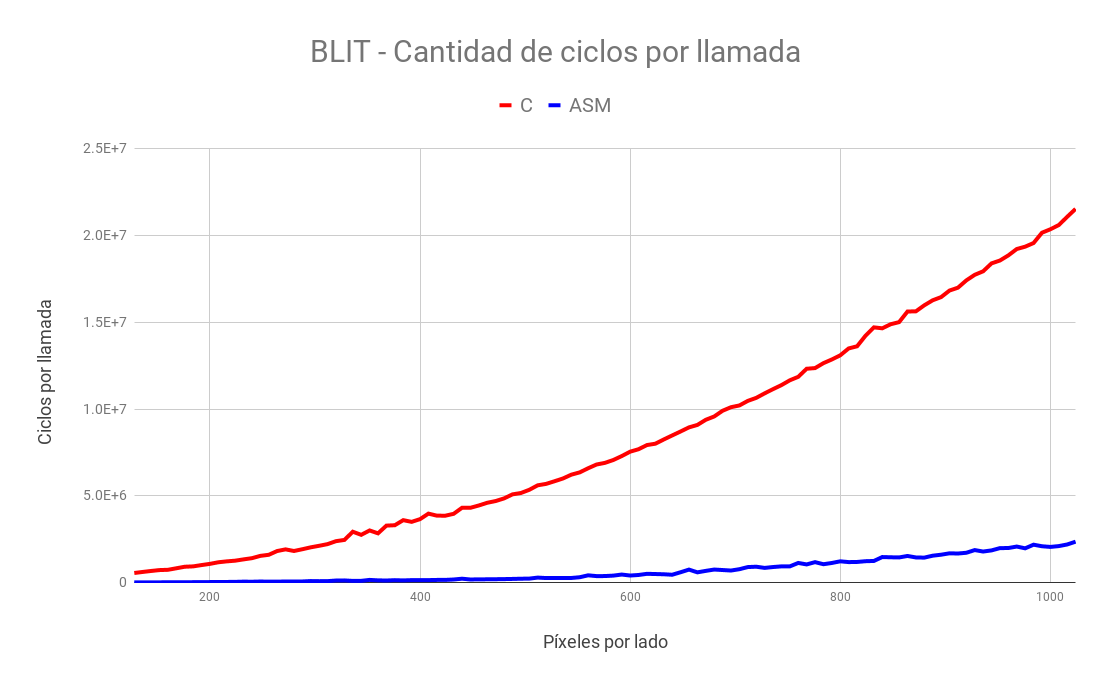
\includegraphics[width=0.45\textwidth]{imagenes/testperformance/BLITperformance.png} &
	  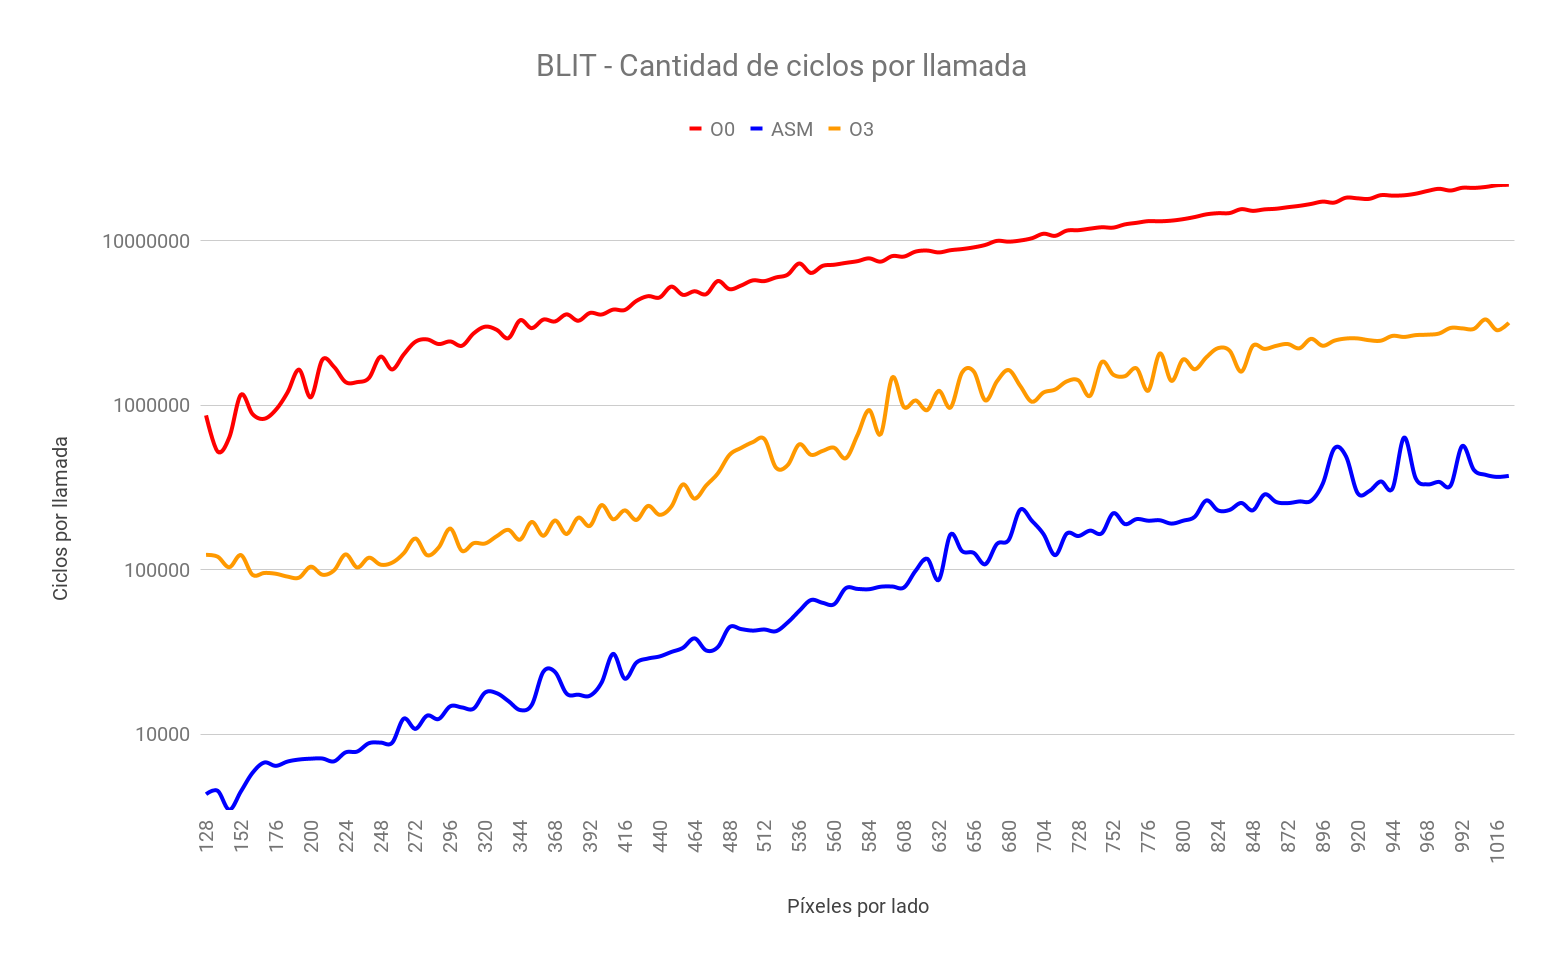
\includegraphics[width=0.45\textwidth]{imagenes/testperformance/BLITperformanceLOG.png} \\
	  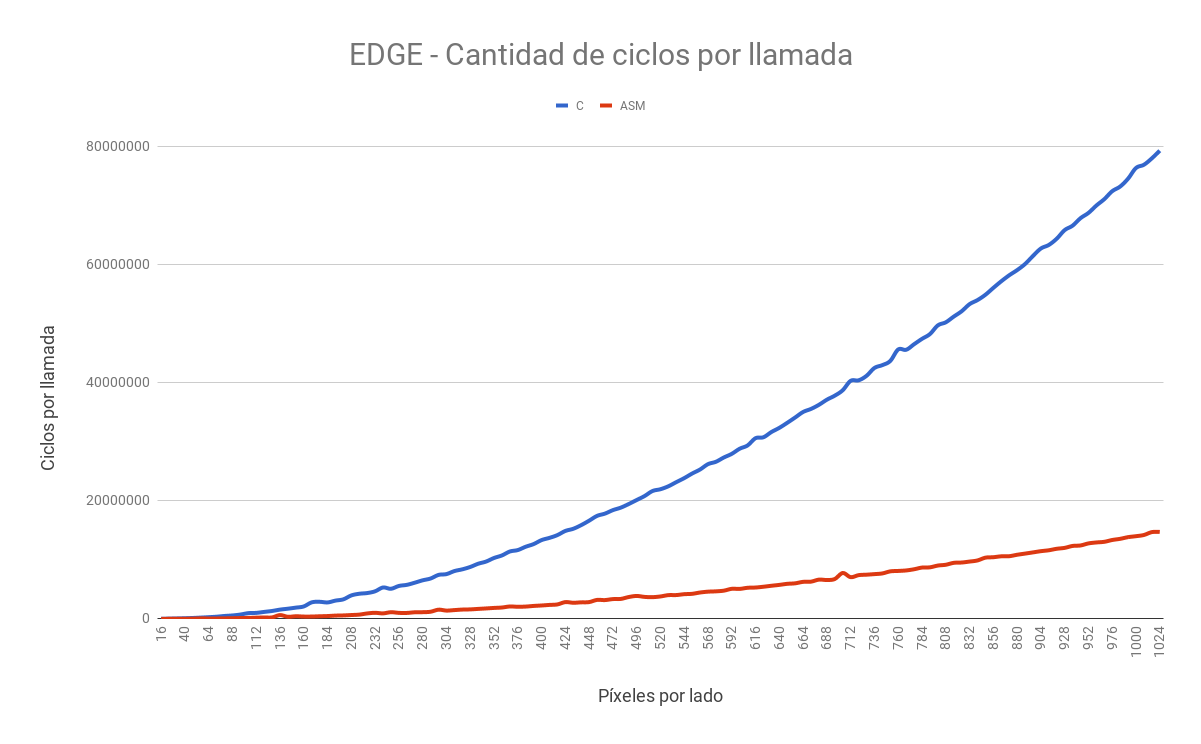
\includegraphics[width=0.45\textwidth]{imagenes/testperformance/EDGEperformanceLIN.png} &
	  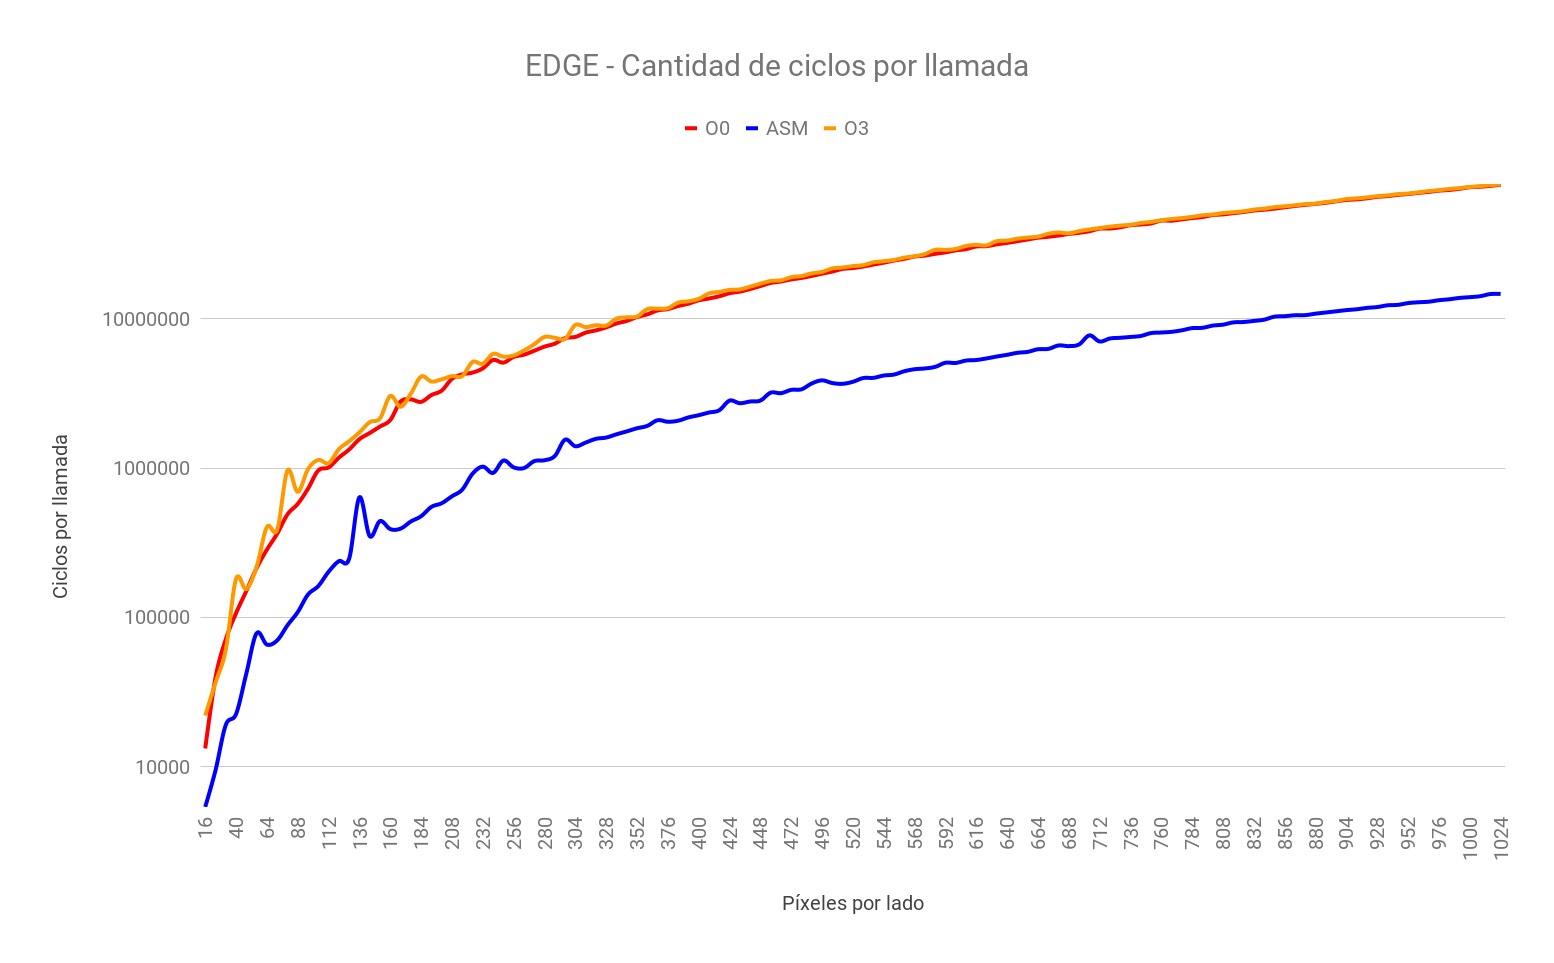
\includegraphics[width=0.45\textwidth]{imagenes/testperformance/EDGEperformanceLOG.png} \\
	  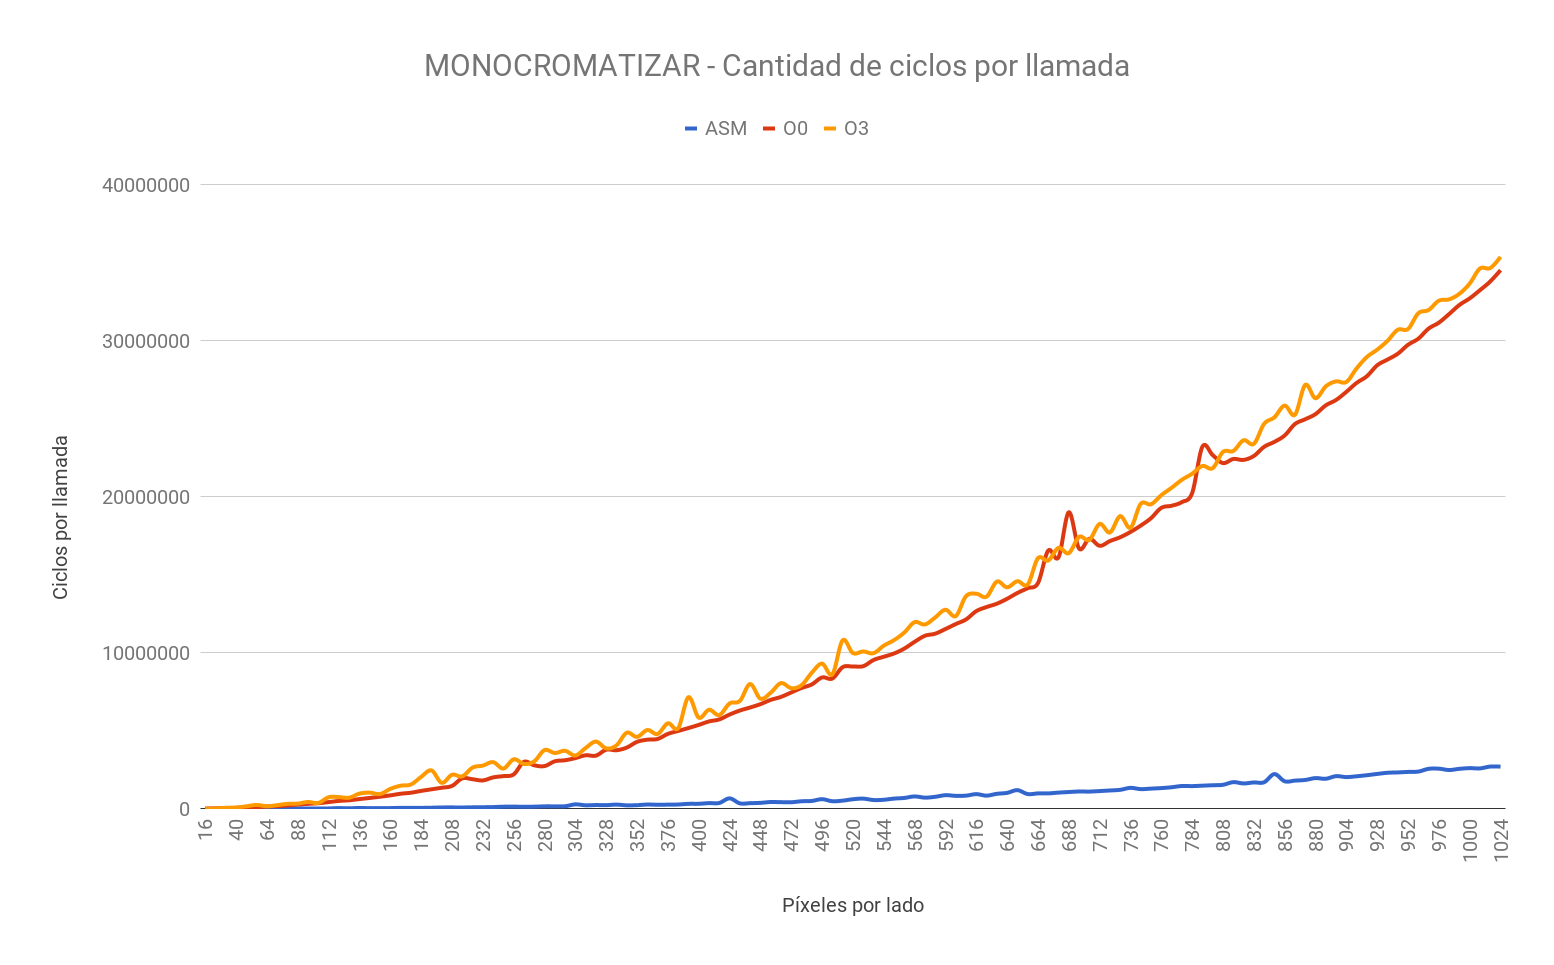
\includegraphics[width=0.45\textwidth]{imagenes/testperformance/MONOperformanceLIN.png} &
	  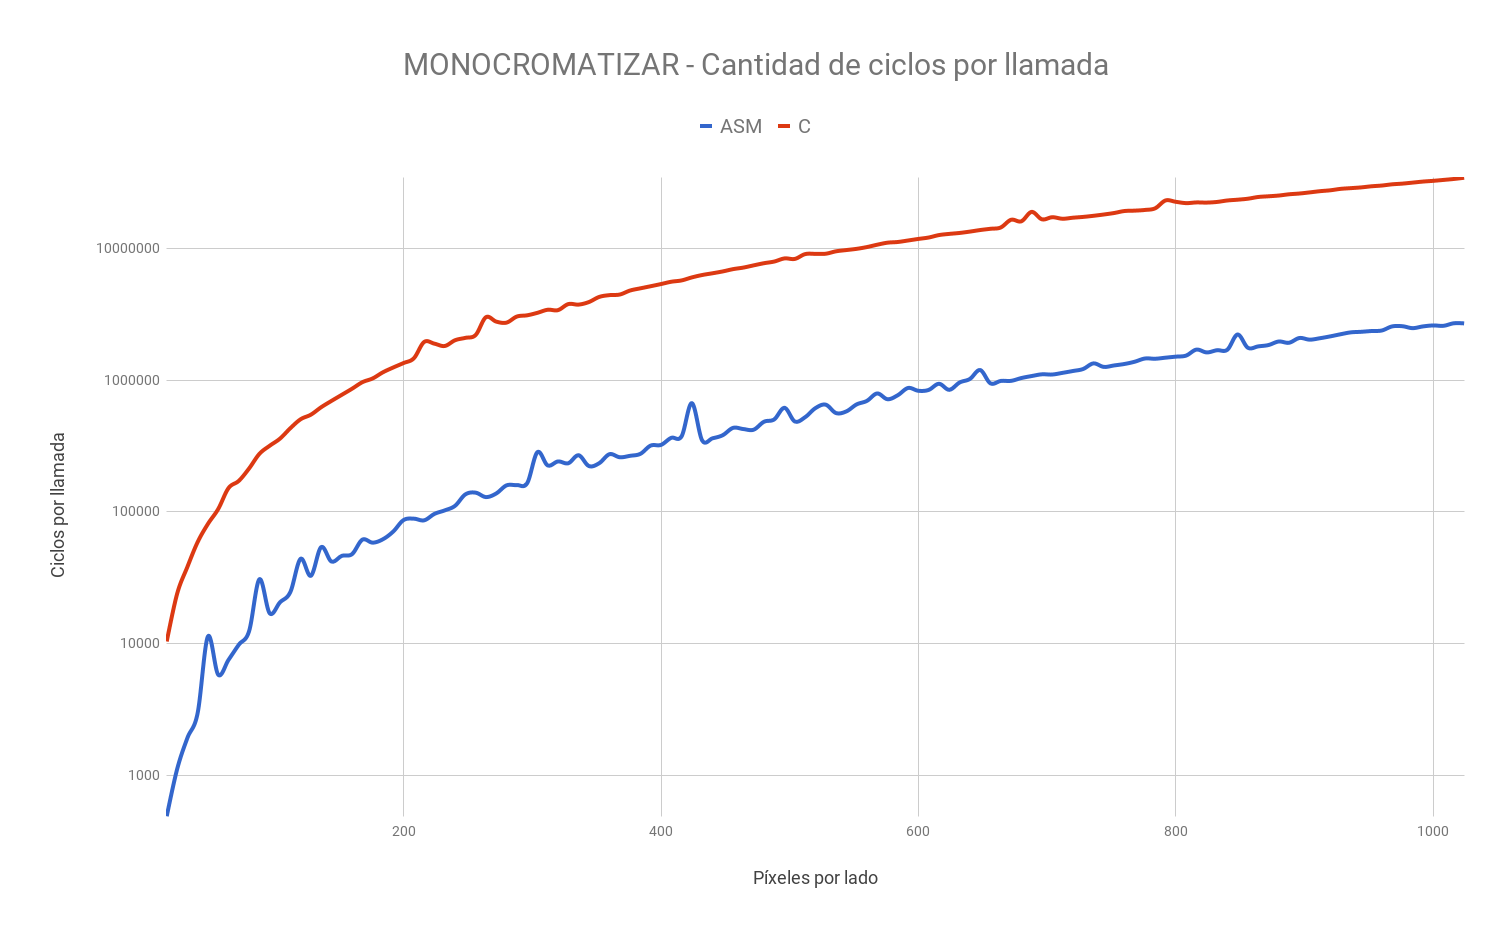
\includegraphics[width=0.45\textwidth]{imagenes/testperformance/MONOperformanceLOG.png} \\
	  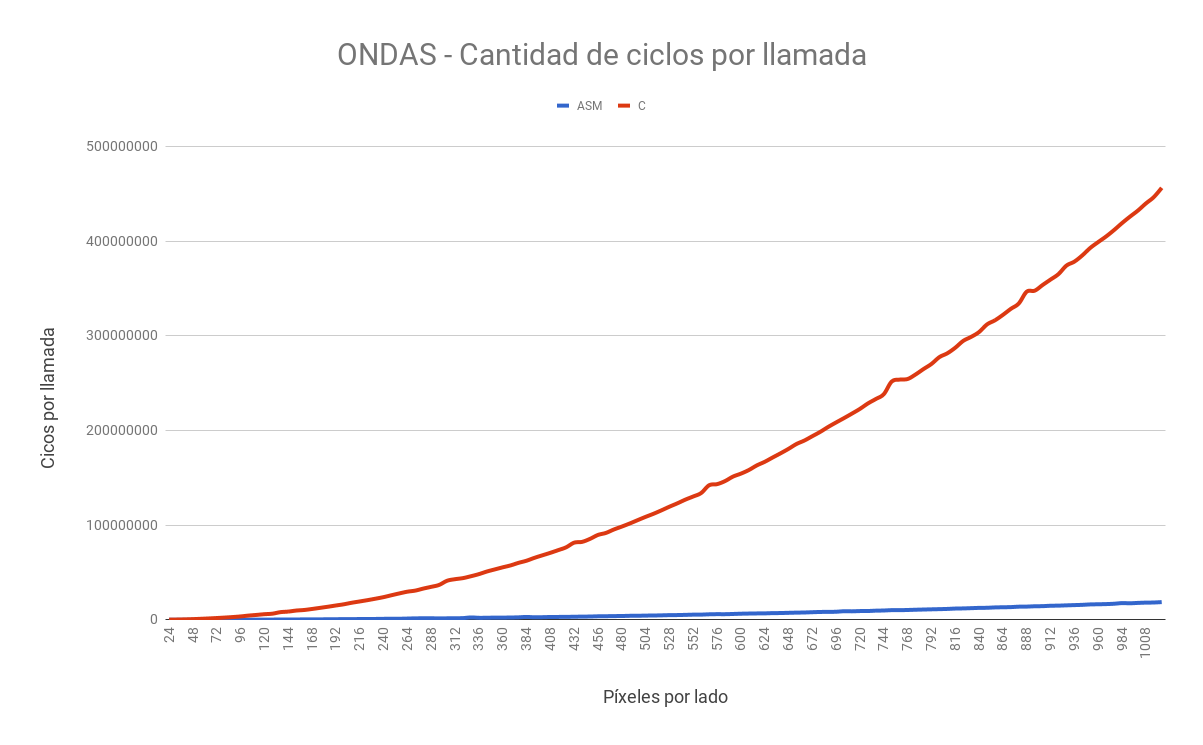
\includegraphics[width=0.45\textwidth]{imagenes/testperformance/ONDASperformanceLIN.png} &
	  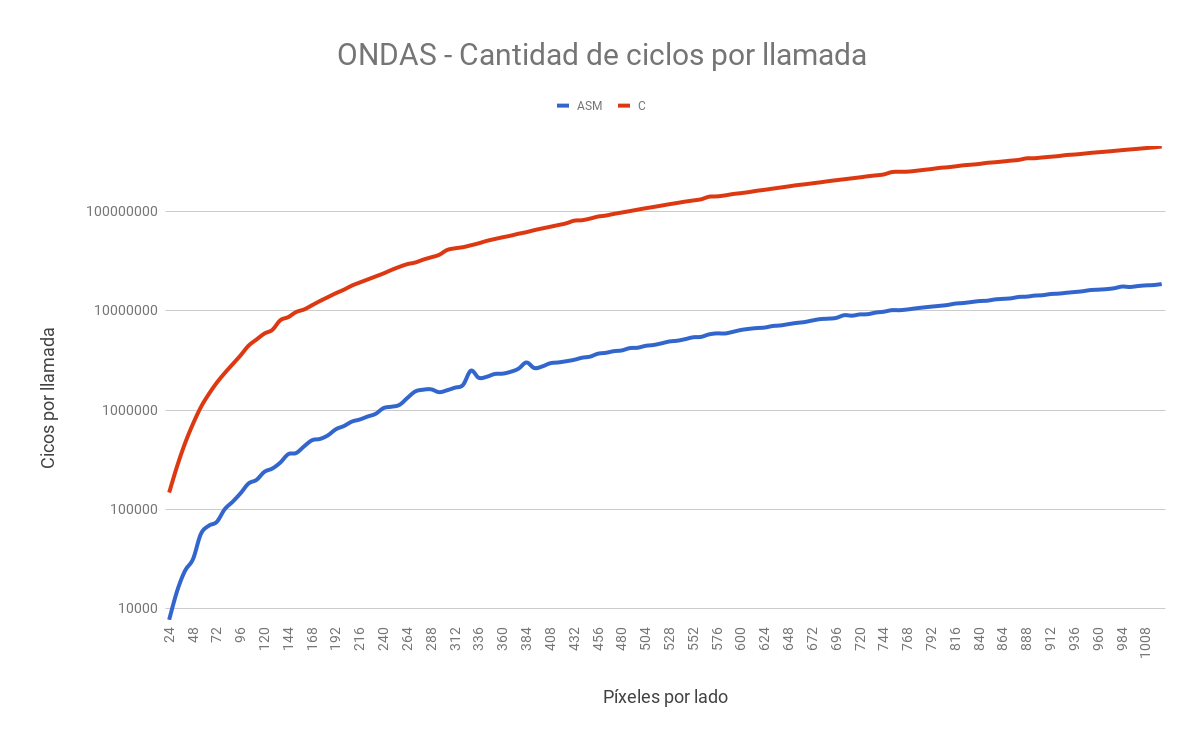
\includegraphics[width=0.45\textwidth]{imagenes/testperformance/ONDASperformanceLOG.png} \\
	  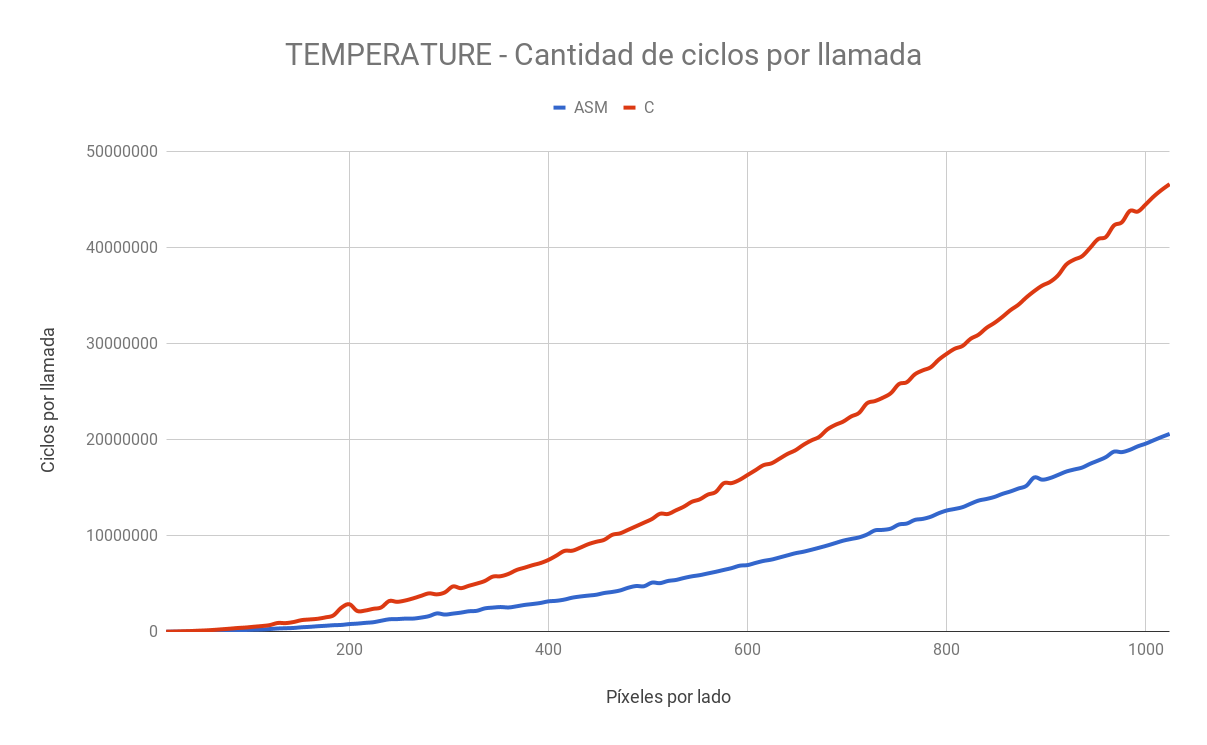
\includegraphics[width=0.45\textwidth]{imagenes/testperformance/TEMPperformance.png} &
	  \includegraphics[width=0.45\textwidth]{imagenes/testperformance/TEMPperformancelog.png} \\
	\end{tabular}
   \end{center}

\subsection{SIMD vs. SISD}

En la misma línea del experimento anterior quisimos evaluar las diferencias de tiempo entre el mismo algoritmo implementado en C, en ASM usando instrucciones SISD y en ASM con SIMD. La reescritura del código utilizando instrucciones SISD requirió 60 líneas de código, usando SIMD 30, y con C apenas 10; el tamaño de los archivos objeto pesó 2592B en SISD, 2608B en SIMD y 4280B en C.

\begin{center}

	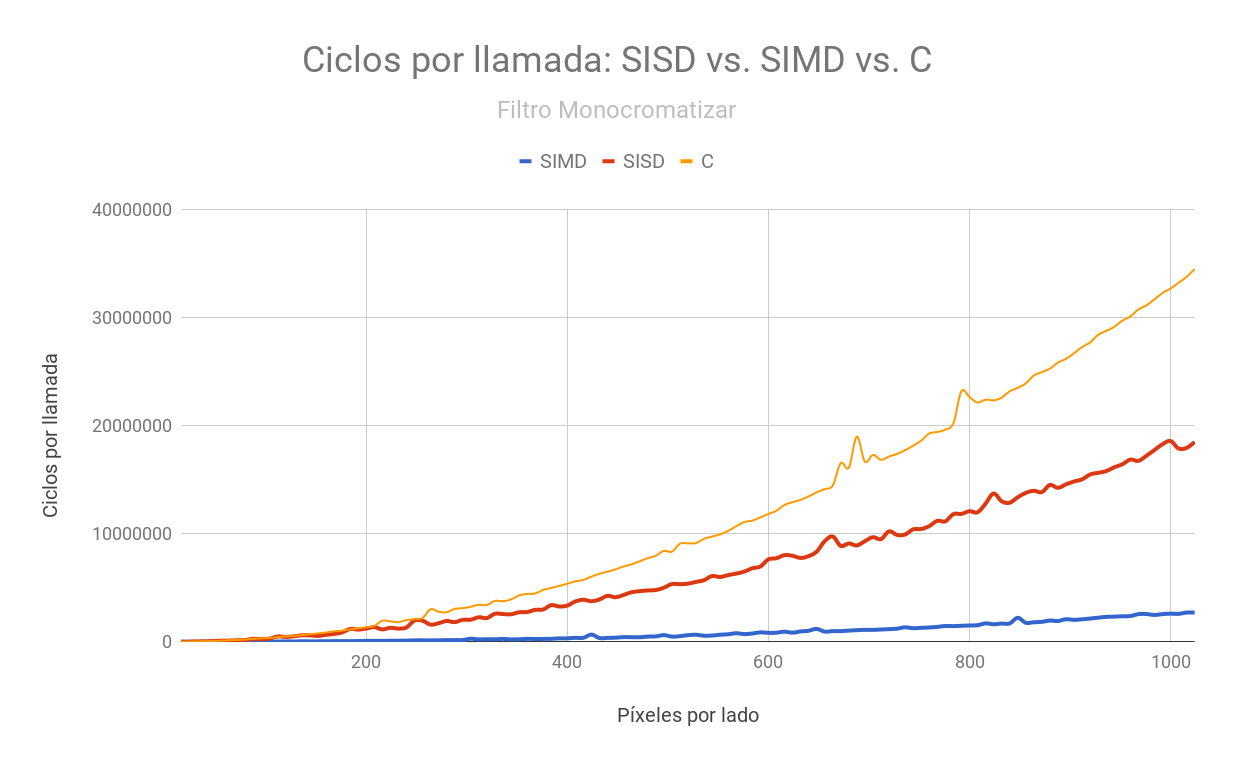
\includegraphics[width=0.9\textwidth]{imagenes/simdsisd/SIMDvsSISDvsClin.png} \\
	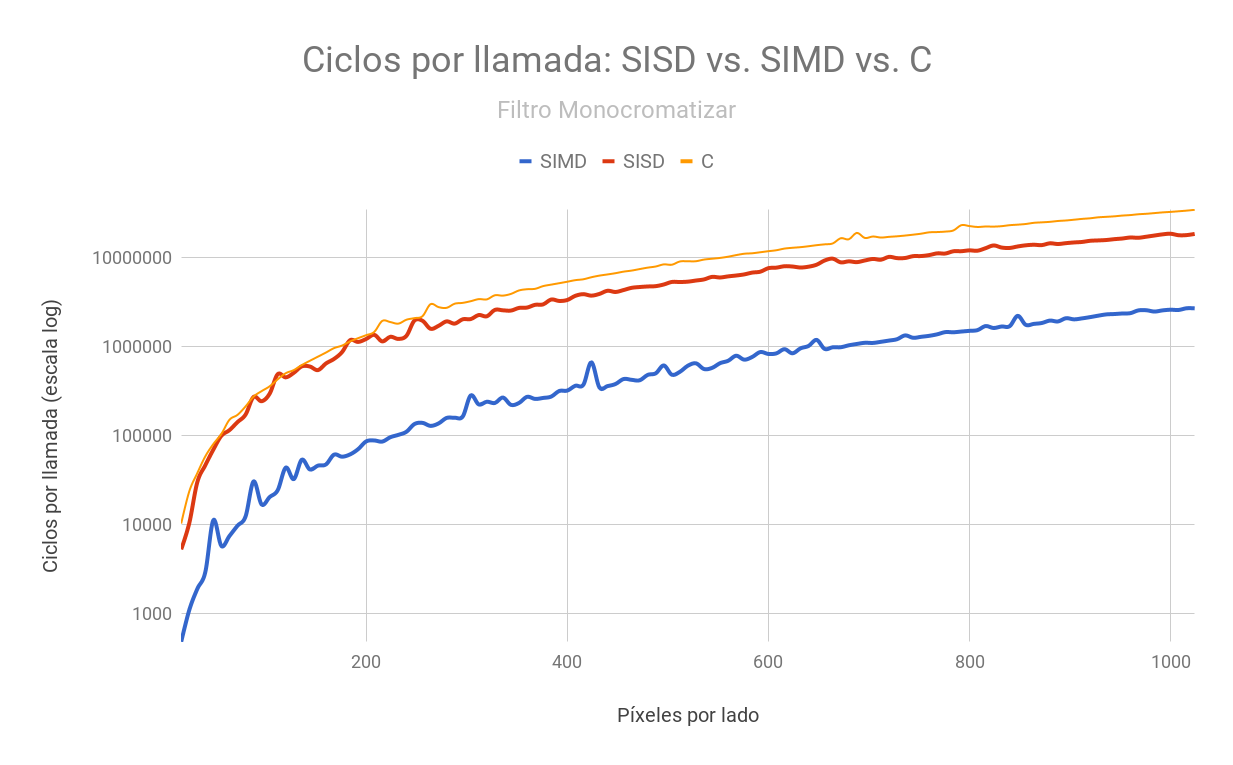
\includegraphics[width=0.9\textwidth]{imagenes/simdsisd/SIMDvsSISDvsClog.png}

\end{center}

Nuevamente pudimos apreciar como las instrucciones SIMD logran una superioridad en performance con respecto a la programación trabajando con datos secuencialmente. El mismo algoritmo implementado utilizando instrucciones SISD no logró imponerse sobre C para imagenes pequeñas -por debajo de los 256 píxeles por lado-, aunque sí lo logró para imagenes de mayor tamaño. En este caso el beneficio de trabajar en ASM puede verse opacado por la facilidad de la programación en C si no se utilizan las instrucciones SIMD. Sin embargo de mantenerse este crecimiento en la cantidad de llamadas para cada implementación, C sigue perdiendo cuando es más exigido.

\subsection{Branch Prediction}

\begin{center}
	\begin{tabular}{cccc}
	  
\includegraphics[width=0.45\textwidth]{imagenes/antiTEMP.jpg} &
	  
\includegraphics[width=0.45\textwidth]{imagenes/random.jpg} \\
	\end{tabular}
   \end{center}

\begin{center}

	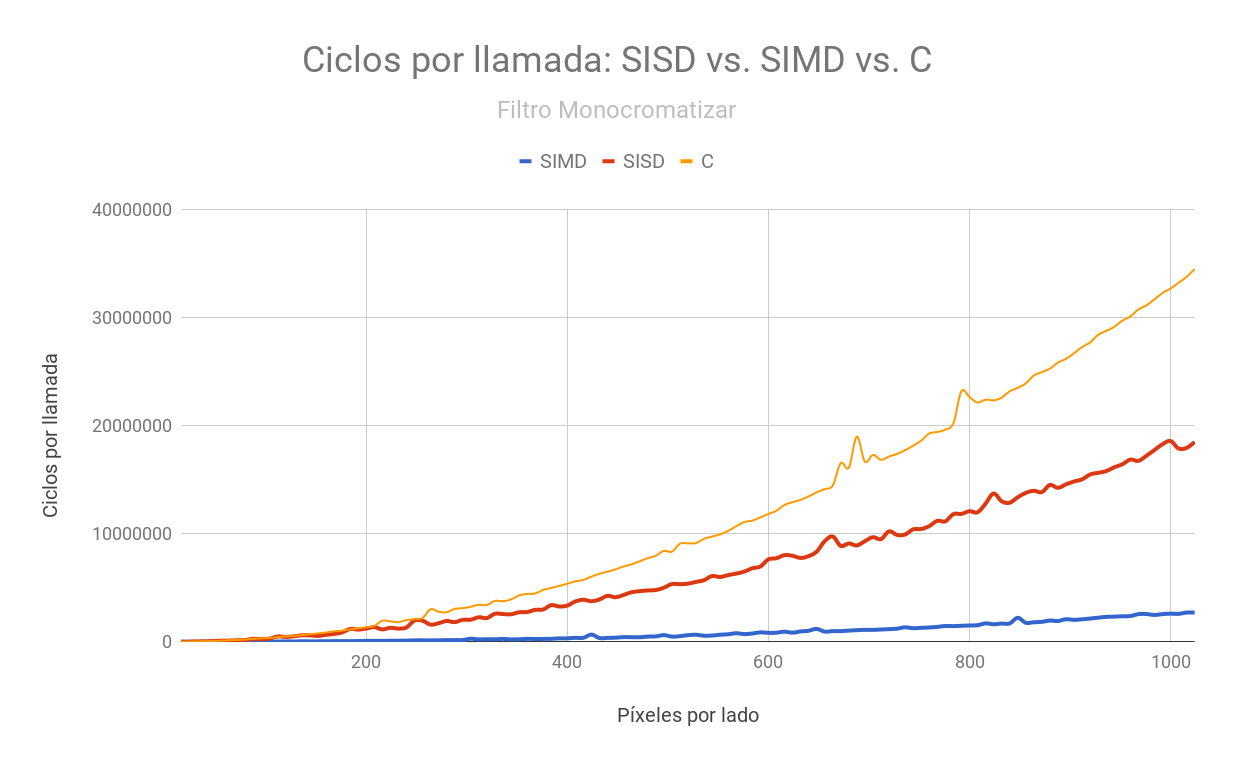
\includegraphics[width=0.9\textwidth]{imagenes/simdsisd/SIMDvsSISDvsClin.png} \\
	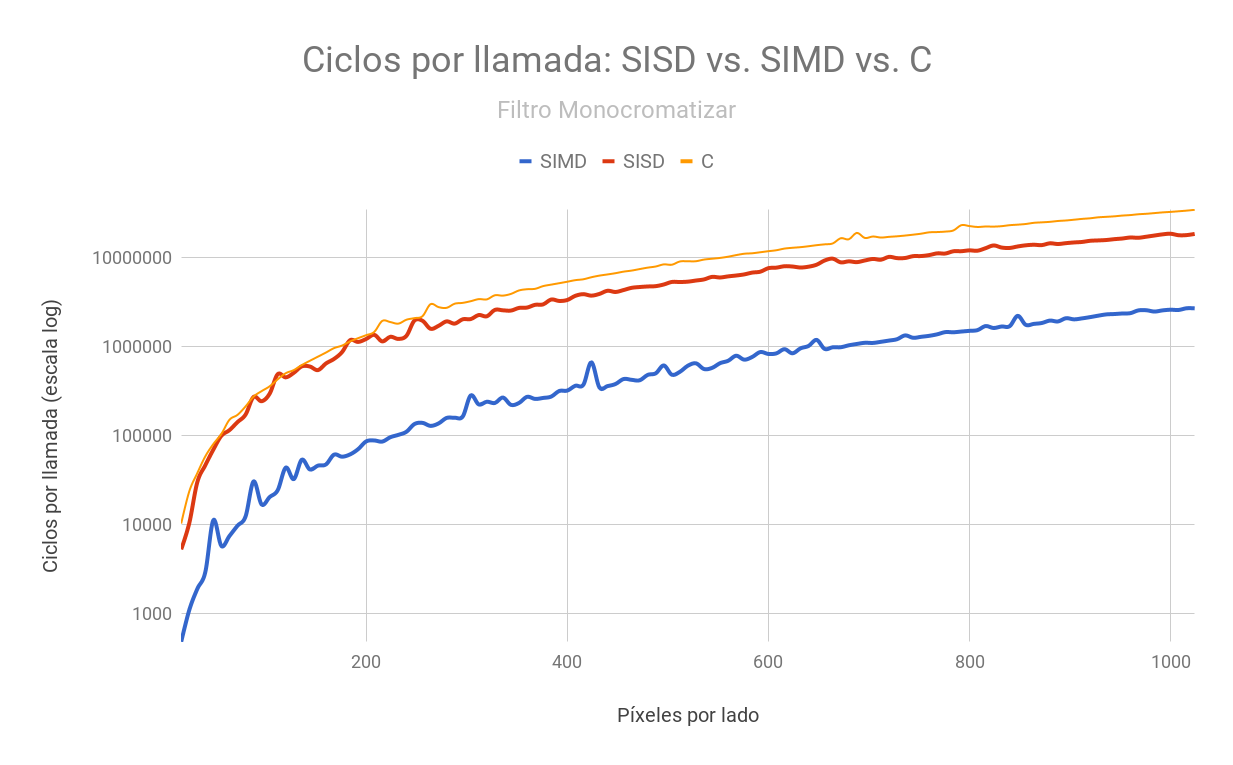
\includegraphics[width=0.9\textwidth]{imagenes/simdsisd/SIMDvsSISDvsClog.png}

\end{center}

\subsection{Loop Unrolling}

\begin{center}

	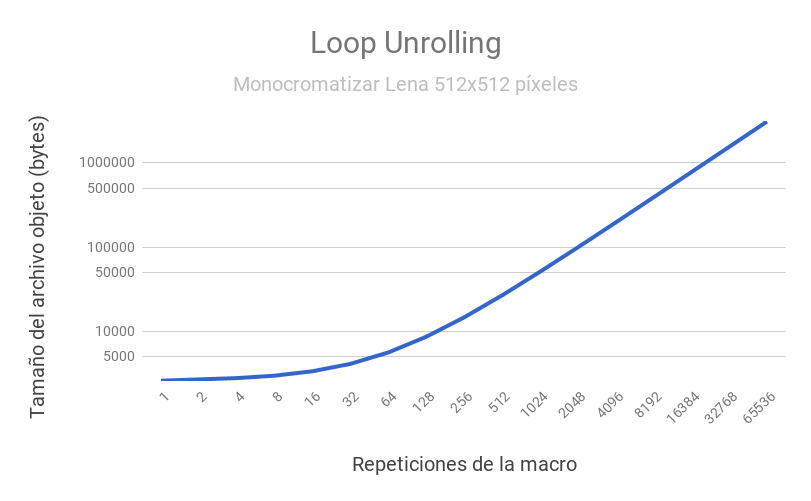
\includegraphics[width=0.9\textwidth]{imagenes/loopunrolling/size.png} \\
	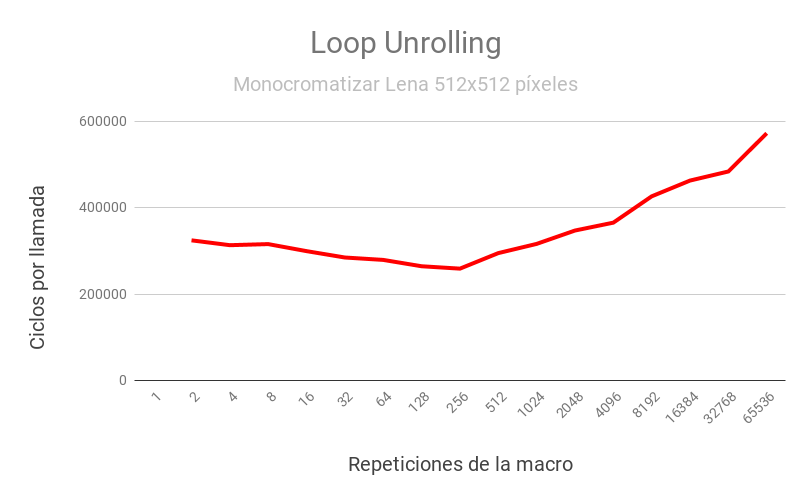
\includegraphics[width=0.9\textwidth]{imagenes/loopunrolling/time.png}

\end{center}

% La forma de medir el rendimiento de nuestras implementaciones se realizará por medio de la toma de tiempos de ejecución del algoritmo (sea este el codigo version asembler o el codigo C). Como los tiempos de ejecución son muy pequeños, se utilizará uno de los contadores de performance que posee el procesador.
% La instrucción de assembler rdtsc permite obtener el valor del Time Stamp Counter (TSC) del procesador. Este registro se incrementa en uno con cada ciclo del procesador. Obteniendo la diferencia entre los contadores antes y después de la llamada a la función, podemos obtener la cantidad de ciclos de esa ejecución. Esta cantidad de ciclos no es siempre igual entre invocaciones de la función, ya que este registro es global del procesador y se ve afectado por una serie de factores. \newline

% Existen principalmente dos problemáticas a solucionar:
% 1). La ejecución puede ser interrumpida por el scheduler para realizar un cambio de contexto,
% esto implicará contar muchos más ciclos (outliers) que si nuestra función se ejecutara sin
% interrupciones.

% 2). Los procesadores modernos varían su frecuencia de reloj, por lo que la forma de medir
% ciclos cambiará dependiendo del estado del procesador.
% \newline

% \textbf{solucion 1):} Para evitar el problema de los ciclos outliers lo que hicimos fue,

% \begin{itemize}
% 	\item[Paso 1:] En nuestro caso hicimos 100 veces la medición de tiempo de nuestro algoritmo y guardarlo en un contenedor(podría ser un arreglo,lista, conjunto, diccionario,.., etc).
% 	\item[Paso 2:] Sacar la media, tambien conocido como promedio, ejemplito:
% 		\begin{center} $ Prom =\frac{x_1+x_2+...+x_{100}}{100}$ \end{center}
% 		Donde $x_i$ es la medición de tiempo de la medición número $i$, con $1 \leq i \leq 100$ 
% 	\item[Paso 3:] Calculamos la varianza: 			
% 				\begin{center}
% 					$Varianza = \sigma^2 = \frac{(x_1 - Prom)+ (x_2 - prom)+ ...+ (x_{100} - prom)}{100} $
% 				\end{center}
% 	\item[Paso 4:] Calculamos el desvio estandar,  $\sigma = \sqrt{Varianza}$
% 	\item[Paso 5:] Utilizando el desvio estandar y el promedio, puedo ver que medición es "buena"  \\ y cual no. Más formalmente una medicion es "buena" si cumple: 
% 					\begin{center}
% 					$Prom - \sigma \leq x_i \leq Prom + \sigma $. %%\newline
% 					\end{center}
% 	 Luego sumando las todas las mediciones  "buenas" \\ y dividiendalas por la cantidad de mediciones buenas, obtengo el "promedio bueno". Con esto amortiguaria la cantidad de outliers de mis mediciones. 			
% \end{itemize}

% \textbf{Observar:} Todo lo anterior sirve también para mas de 100 mediciones. \newline

% \textbf{Solucion 2):} La solución que planteamos para esto fue, ejecutar sólamente el algoritmo. Con esto queremos decir que la ejecución estara en el nivel más alto de privilegio de ejecución. Esto lo hacemos metiendonos en el sistema operativo (en este caso ubuntu 14.04), tocando el monitor de sistema para darle privilegio a la ejecución. Tambien evitamos interumpir la maquina de forma mecanica(osea humana).  
